\documentclass[12pt]{report}

\usepackage{hyperref}
\usepackage{fontspec}
\usepackage{polyglossia}
\usepackage{xcolor} 
\usepackage{graphicx}
\usepackage[final]{pdfpages}

\linespread{1.2}
\widowpenalty=10000
\clubpenalty=10000
\raggedbottom
\sloppy
\lefthyphenmin=2
\righthyphenmin=2
\setdefaultlanguage{malayalam}
\setmainfont[Script=Malayalam,HyphenChar="00AD]{Gayathri}


\usepackage{color}
\usepackage{xcolor}
\definecolor{dark-red}{rgb}{0.4,0.15,0.15}
\definecolor{dark-blue}{rgb}{0.15,0.15,0.8}
\definecolor{medium-blue}{rgb}{0,0,0.5}
\definecolor{offwhite}{rgb}{1,.98,.94}
\hypersetup{
	colorlinks, linkcolor={dark-blue},
	citecolor={dark-blue}, urlcolor={medium-blue}
}


\begin{document}
	
\begin{titlepage}
	\pagecolor{offwhite}\afterpage{\nopagecolor}
	\begin{center}
		\begin{centering}
		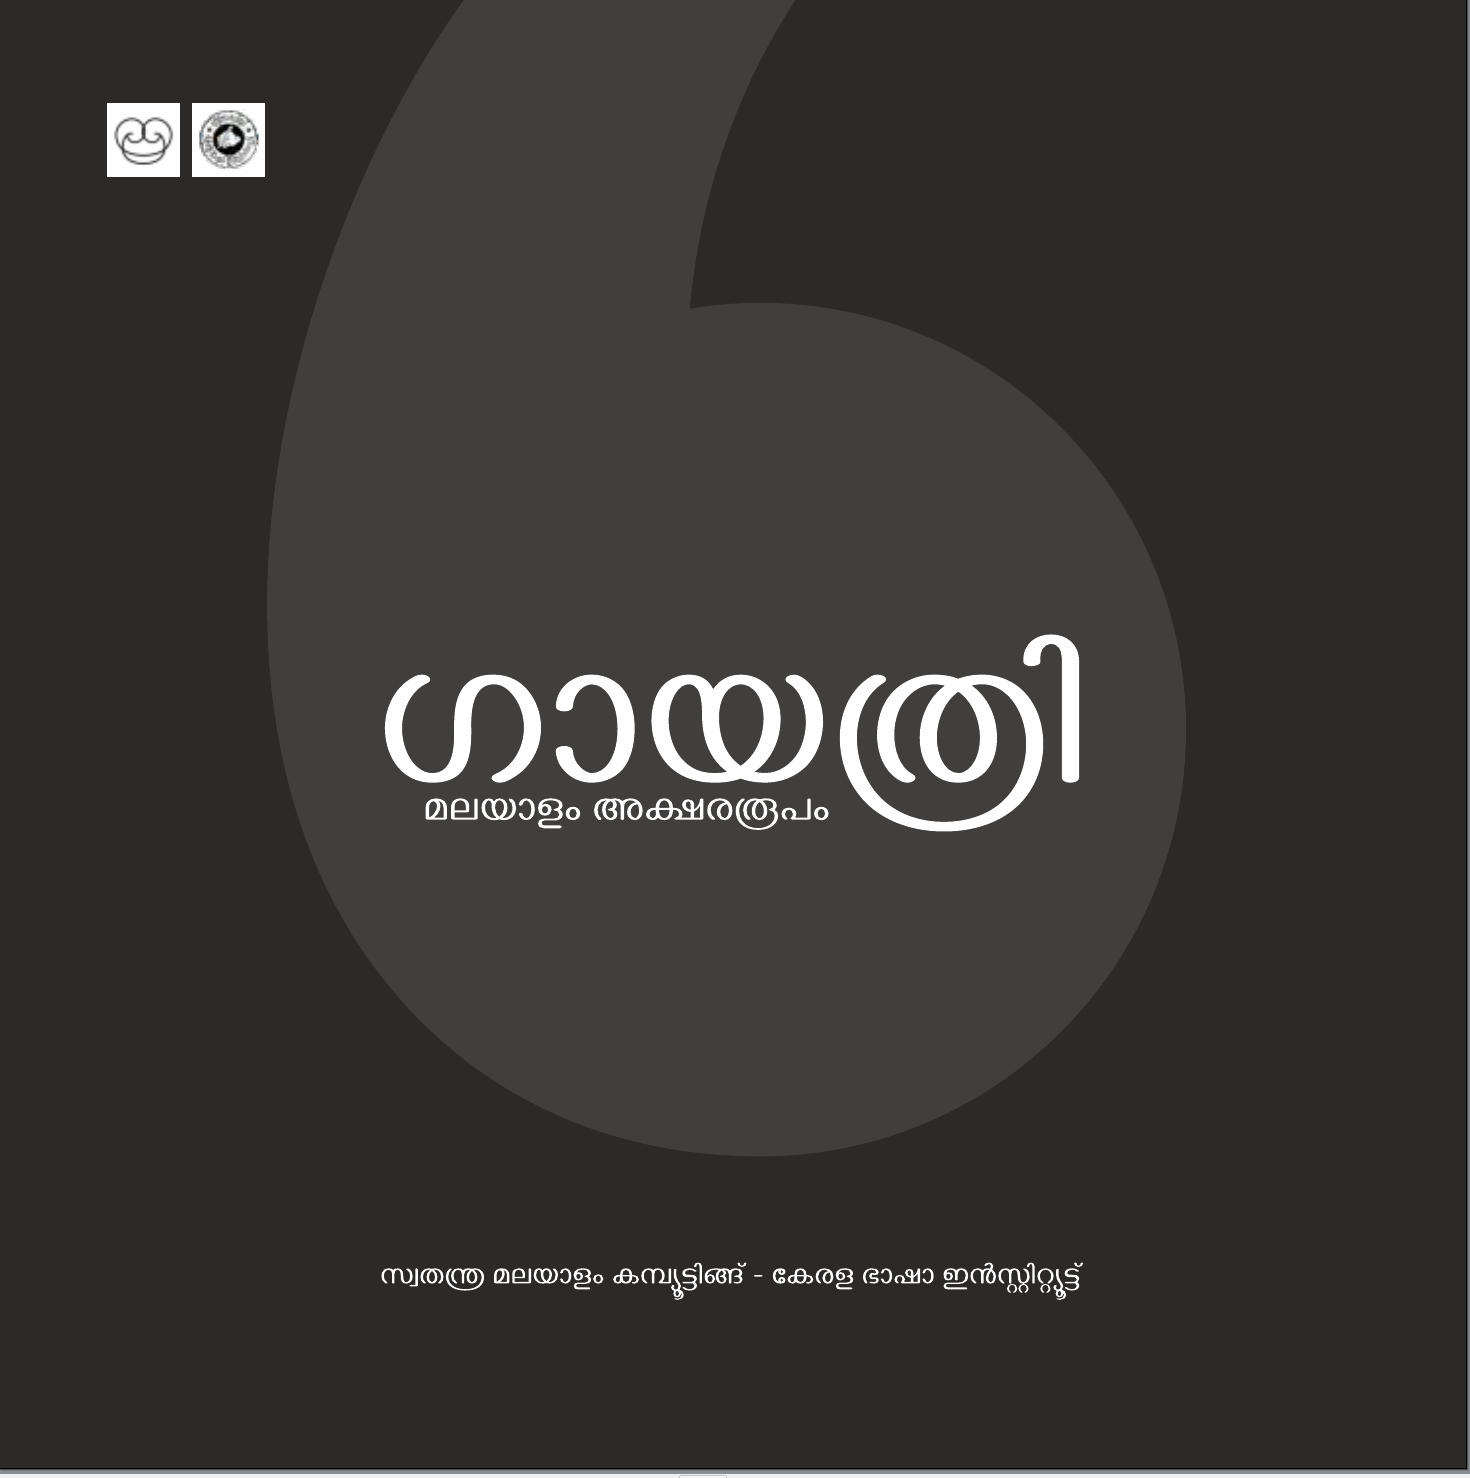
\includegraphics[width=\textwidth]{title.png}\\[0.5cm]	
		\end
		{centering}
		

		\textsc{\Large {സ്വതന്ത്ര മലയാളം കമ്പ്യൂട്ടിങ്ങ്}}~\\
		
		{\textsc{\Large {പ്രോജക്ട് റിപ്പോര്‍ട്ട്}}}\\
		2018
	\end{center}
\end{titlepage}
 

\thispagestyle{empty}	
\clearpage
	
	\chapter*{ആമുഖം}
	

	കേരള ഭാഷാ ഇന്‍സ്റ്റിറ്റ്യൂട്ടിന്റെ സാമ്പത്തിക സഹായത്തോടെ സ്വതന്ത്ര മലയാളം കമ്പ്യൂട്ടിങ്ങ് നിര്‍മ്മിച് മലയാളം യൂണിക്കോഡ് അക്ഷരരൂപമാണ്  \textbf{ഗായത്രി}. അക്ഷരങ്ങളുടെ  രൂപകല്പന നിർവഹിച്ചത് ബിനോയ് ഡൊമിനിക്ക് ആണ്. ഓപ്പണ്‍ടൈപ്പ് സാങ്കേതികതയിൽ കാവ്യ മനോഹർ പ്രവർത്തിച്ചു. പ്രോജക്ട് മേല്‍നോട്ടം സന്തോഷ് തോട്ടിങ്ങൽ നിർവ്വഹിച്ചു.
	
	\paragraph{}
	റെഗുലര്‍, ബോള്‍ഡ്, തിന്‍ എന്നിങ്ങനെ മൂന്നു കനങ്ങളിലുള്ള ഫോണ്ടുകളായി ലഭ്യമായ ഗായത്രി, തലക്കെട്ടുകള്‍ക്ക് അനുയോജ്യമായ വിധമാണ് രൂപകല്പന ചെയ്തിരിക്കുന്നത്. എങ്കിലും ചെറിയ വലിപ്പത്തിലും സാമാന്യം നല്ല വായനാക്ഷമത ഗായത്രിയ്ക്കുണ്ട്. ഈ റിപ്പോര്‍ട്ട് പൂര്‍ണ്ണമായും ഗായത്രി  ഉപയോഗിച്ചാണ് തയ്യാറാക്കിയിരിക്കുന്നത്.
	
\thispagestyle{empty}
\clearpage
	\chapter*{ അക്ഷരസഞ്ചയം}
	

	
	യൂണിക്കോഡിന്റെ പതിനൊന്നാം പതിപ്പിനെ ആധാരമാക്കിയാണ് ഗായത്രി നിര്‍മ്മിച്ചിട്ടുള്ളത്. മലയാളത്തില്‍ ഇന്ന് നിത്യോപയോഗത്തിലുള്ള സ്വരങ്ങളും വ്യഞ്ജനങ്ങളും ചില്ലക്ഷരങ്ങളും അക്കങ്ങളും കൂടാതെ പ്രാചീനമലയാളത്തില്‍ നിലനിന്നിരുന്ന അക്ഷരങ്ങളും അക്കങ്ങളുമെല്ലാം ചേര്‍ന്ന സമഗ്രമായ അക്ഷരസഞ്ചയം ഗായത്രിയിലുണ്ട്. മലയാളത്തിലെ പുരാരേഖകള്‍ ഡിജിറ്റൈസ് ചെയ്യുമ്പോള്‍ അത്യന്താപേക്ഷിതമാണിവ. കാല്‍, അര, മുക്കാല്‍, പതിനാറില്‍മൂന്ന് തുടങ്ങിയ ഭിന്നസംഖ്യാരൂപങ്ങളെ കുറിക്കുന്ന ൳, ൴, ൵, ൸ ചിഹ്നങ്ങളൊക്കെ ഗായത്രിയിലുണ്ട്. മലയാളം യൂണിക്കോഡ് പട്ടിക സമ്പൂർണ്ണമായി ഗായത്രിയിൽ തയ്യാറാക്കിയിരിക്കുന്നത് ചിത്രം \ref{unicode} ല്‍ കാണാം.
	
	\begin{figure}
		\begin{centering}
			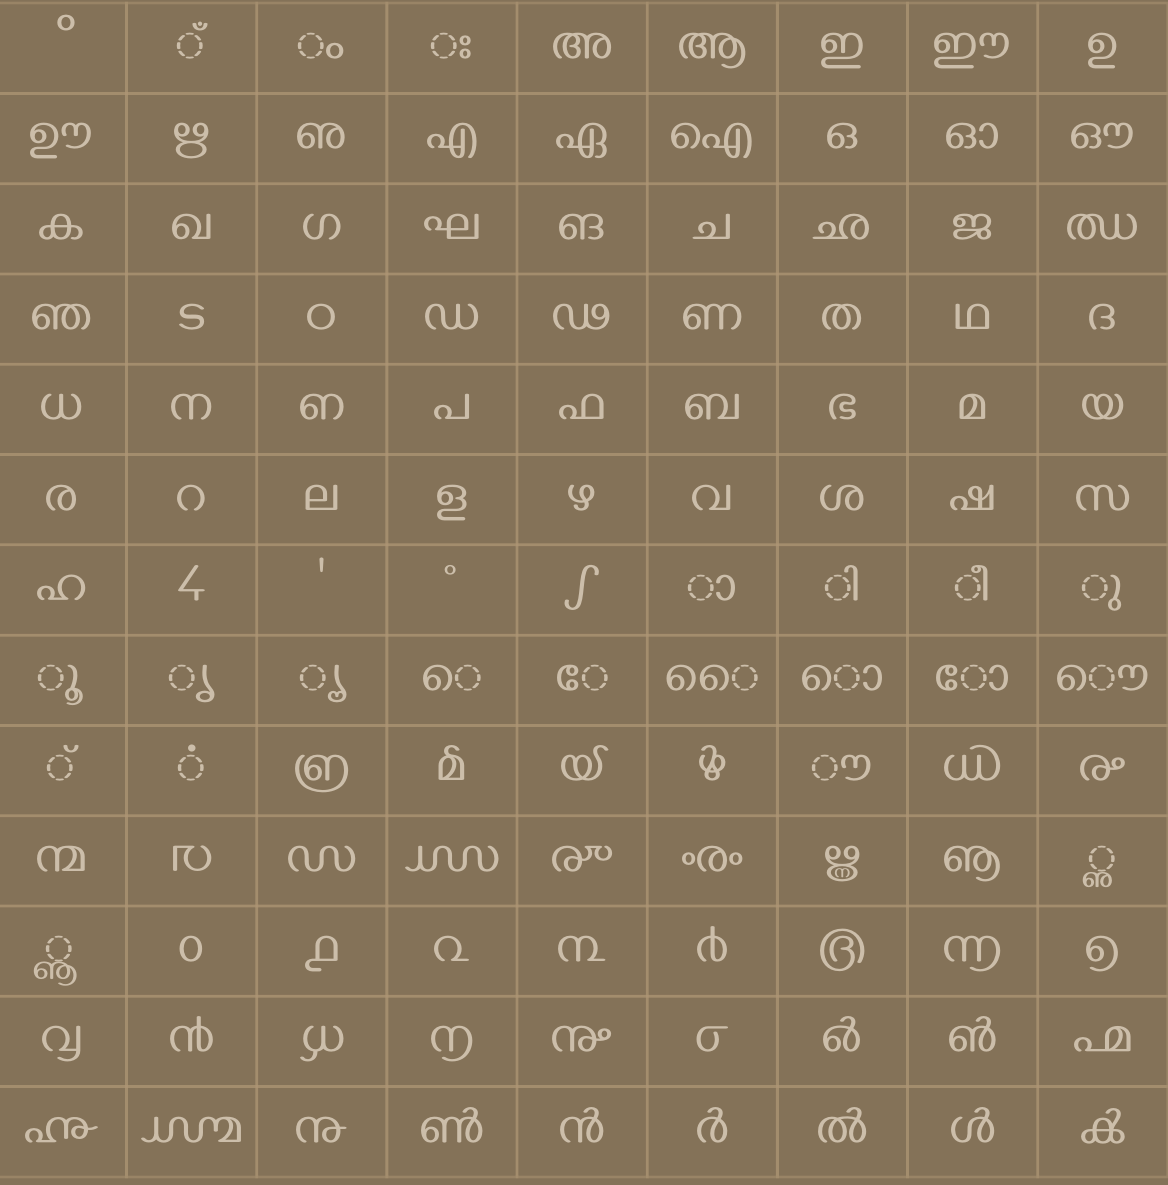
\includegraphics[width=0.8\textwidth]{ml-unicode.png}
			\caption{മലയാളം യൂണിക്കോഡ് സമ്പൂര്‍ണ്ണ കവറേജ്}
			\label{unicode}
		\end{centering}
	\end{figure}
	
	\paragraph{}
	മലയാളത്തിലെ കൂട്ടക്ഷരങ്ങളെ പരമാവധി ഉള്‍ക്കൊള്ളിച്ചുകൊണ്ടാണ് ഗായത്രിയുടെ രൂപകല്പന‍. അതുകൊണ്ട് തന്നെ ഇതിനെ ഒരു സമഗ്രലിപി ഫോണ്ടെന്ന് വിളിക്കാം.
	
	\paragraph{}
	ഇന്ന് മലയാളരേഖകളില്‍ മലയാളത്തോടൊപ്പം ഇംഗ്ലീഷ് വാക്കുകളും കലര്‍ത്തിയെഴുതുന്നത് സര്‍വ്വ സാധാരണമാണ്. അതുകൊണ്ട് തന്നെ ആധുനികമലയാളം ഫോണ്ടുകളില്‍ മലയാളം ലിപിയുടെ ശൈലിയ്ക്ക് അനുരൂപമായ ഇംഗ്ലീഷുള്‍പ്പെടുന്ന ലാറ്റിന്‍ അക്ഷരങ്ങളും അത്യാവശ്യമാണ്. ഗായത്രി ഫോണ്ടില്‍ ലാറ്റിന്‍ അക്ഷരങ്ങളും കൂടി അതുകൊണ്ടു തന്നെ ഉള്‍പ്പെടുത്തിയിട്ടുണ്ട്.  എല്ലാം ചേര്‍ന്ന് ആകെ ആയിരത്തി ഒരുന്നൂറിൽപ്പരം അക്ഷരരൂപങ്ങൾ‍ ഗായത്രിയിലുണ്ട്. 
	
	\paragraph{}
	മലയാളത്തിലെ ചില അക്ഷരങ്ങള്‍ക്ക് സാര്‍വ്വത്രികമായി ഒരേ രൂപമല്ല ഉള്ളത്. 'ച്ച', 'കൂ', 'ള്ള' തുടങ്ങിയവയുടെ ശൈലീഭേദങ്ങളുള്‍ക്കൊണ്ടുകൊണ്ട് അവ കൂടി ഗായത്രി ഫോണ്ടില്‍ ചേര്‍ത്തിട്ടുണ്ട്. സോഫ്റ്റ്‌വെയര്‍ സഹായത്തോടെ ഇതിലേതുവേണമെന്നു തെരഞ്ഞെടുക്കാന്‍ ഉപയോക്താവിനാകും. ചിത്രം \ref{style} കാണുക. 
	‍ 
	\begin{figure}
		\begin{centering}
			
\includegraphics[width=0.8\textwidth]{style.jpg}
			\caption{കൂ, ച്ച, ള്ള എന്നിവയുടെ ശൈലീഭേദങ്ങൾ ചിത്രീകരിച്ചിരിക്കുന്നു.}
			\label{style}
		\end{centering}
	\end{figure}
	
	
	\chapter*{രൂപകല്പന}
	
	ആമുഖത്തില്‍ സൂചിപ്പിച്ചത് പോലെ തലക്കെട്ടുകള്‍ക്ക് അനുയോജ്യമായ വിധമാണ് ഗായത്രിയുടെ രൂപകല്പന‍. അക്ഷരങ്ങളിലെ വരകൾക്ക് ഒരേ വീതിയല്ല. അക്ഷരങ്ങളുടെ അറ്റങ്ങള്‍ ഏതാണ്ട് ഉരുണ്ടിട്ടാണ്. കൂർത്ത അറ്റങ്ങൾ ഇല്ലാത്തതുകൊണ്ട് വായന ആയാസരഹിതമായി നടക്കുകയും ചെയ്യും.  വലിയ രൂപത്തില്‍ ഇവ വ്യക്തമായി കാണാവുന്ന മിഴിവാര്‍ന്ന ഡിസൈന്‍ സാദ്ധ്യതകള്‍ ഗായത്രിയ്ക്ക് നല്‍കാനാകും.  ചിത്രം \ref{one} നോക്കുക.
	
	\begin{figure}
		\begin{centering}
			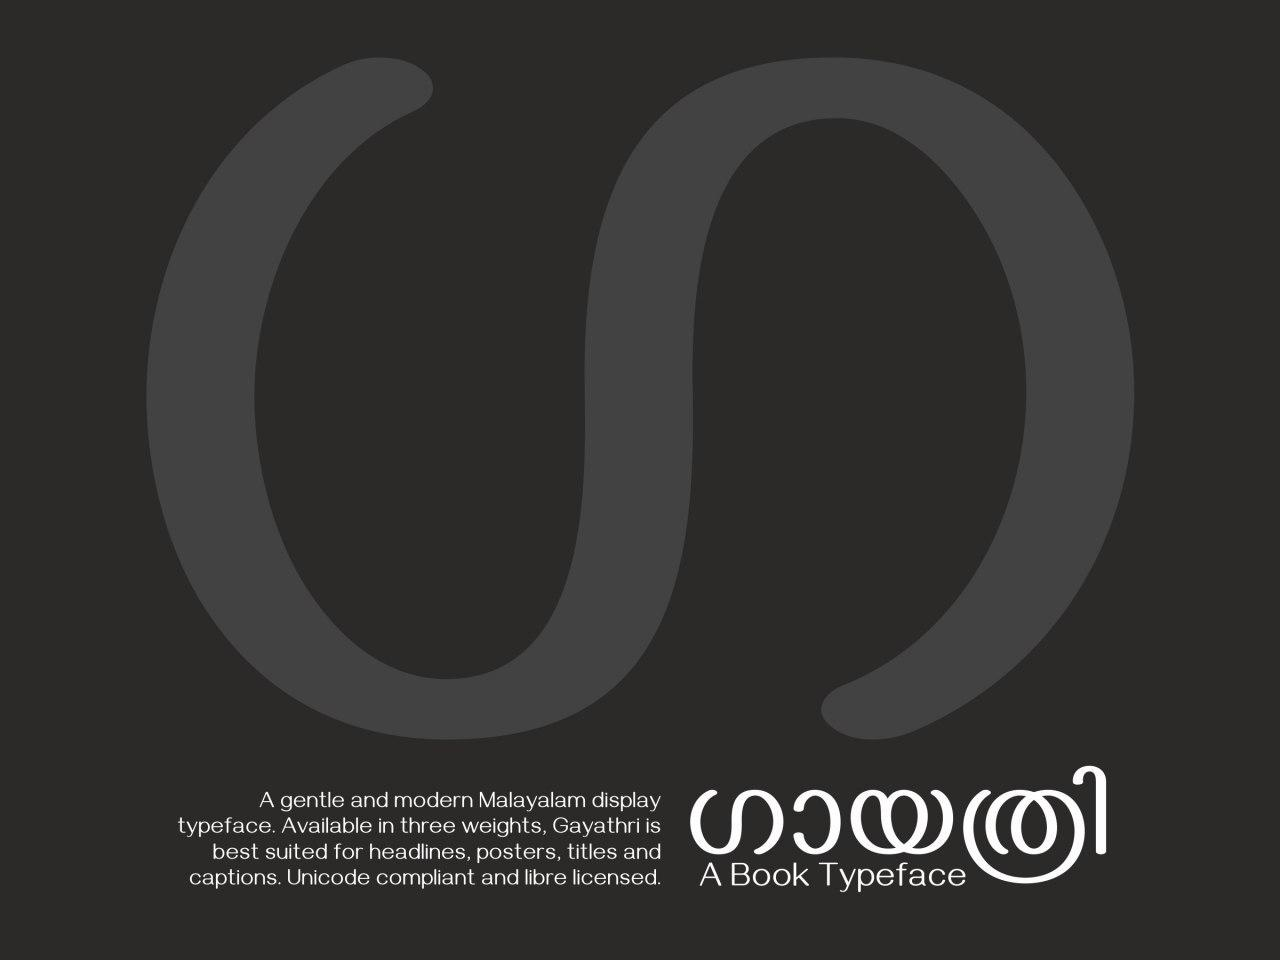
\includegraphics[width=0.8\textwidth]{ga.jpg}
			\caption{ഡിസൈന്‍ വിശദാംശങ്ങള്‍. അക്ഷരങ്ങളുടെ അറ്റങ്ങൾ ഉരുണ്ടതും വായനാസുഖം നൽകുന്നതുമാണ്.}
			\label{one}
		\end{centering}
	\end{figure}
	
	\paragraph{}
	പുസ്തകങ്ങളുടേയും ആനുകാലികങ്ങളുടേയുമെല്ലാം ലേയൗട്ട് തയ്യാറാക്കുമ്പോള്‍ പല കനത്തിലുള്ള ഫോണ്ട് വേരിയന്റുകള്‍ ആവശ്യമായി വരാറുണ്ട്. ഇതിനായി മൂന്നുകനങ്ങളില്‍ - ബോള്‍ഡ്, റെഗുലര്‍, തിന്‍- ഗായത്രി അക്ഷരരൂപങ്ങള്‍ ലഭ്യമാണ്. 
	
	\chapter*{നിര്‍മ്മാണവും ലൈസന്‍സിങ്ങും}
	
	ഗായത്രി ഫോണ്ട് നിര്‍മ്മാണം പൂര്‍ണ്ണമായും സ്വതന്ത്രസോഫ്റ്റ്‌വെയർ ഉപയോഗിച്ചാണ് നിർമ്മിച്ചിരിക്കുന്നത്. ഡിസൈനര്‍ അക്ഷരങ്ങളുടെ ബോള്‍ഡ്, റെഗുലര്‍, തിന്‍ ശൈലികളിലുള്ള വെക്ടര്‍ ഇമേജുകള്‍ തയ്യാറാക്കി. ഫോണ്ടിന്റെ മൂലരൂപം UFO (Unified Font Object) ഫോര്‍മാറ്റിലാണ്. അക്ഷരങ്ങളുടെ വെക്ടർ ചിത്രങ്ങളെ UFO മാതൃകയിലുള്ള ഗ്ലിഫ് ഫയലുകള്‍ ആക്കുകയാണ് ഫോണ്ട് എഞ്ചിനീയറിങ്ങിലെ ആദ്യ പടിയായി ചെയ്തത്. പിന്നീട് കൂട്ടക്ഷരങ്ങള്‍ കൃത്യമായി ചിത്രീകരിക്കാനാവശ്യമായ ഓപ്പണ്‍ടൈപ്പ് നിയമങ്ങള്‍ ചേര്‍ത്ത്  OTF, TTF, WOFF ഫോര്‍മറ്റിലുള്ള ഫോണ്ടുകള്‍ നിര്‍മ്മിച്ചു. ഈ ഫോര്‍മാറ്റുകളിലെല്ലാമുള്ള ഗായത്രിയുടെ ബോള്‍ഡ്, റെഗുലര്‍, തിന്‍ ഫോണ്ടുകള്‍ സ്വതന്ത്ര മലയാളം കമ്പ്യൂട്ടിങ്ങിന്റെ (\url{https://smc.org.in/fonts/}) വെബ്സൈറ്റിൽ നിന്നും ഡൗണ്‍ലോഡ് ചെയ്യാന്‍ ലഭ്യമാണ്.
	
	\paragraph{}
	ഫോണ്ടിന്റെ സോഴ്സ് കോഡ് സ്വതന്ത്രമാണ്. അതായത്, വരച്ച അക്ഷരരൂപങ്ങളുടെ വെക്ടര്‍ ഇമേജുകള്‍ (svg format), ഇവയില്‍ നിന്നും തയ്യാറാക്കിയ ഗ്ലിഫ് ഫയലുകള്‍, ഓപ്പണ്‍ടൈപ്പ്  നിയമങ്ങള്‍ ഇവയെല്ലാം നിര്‍മ്മാണഘട്ടത്തില്‍ ഇതുവരെ വരുത്തിയ മാറ്റങ്ങളുള്‍പ്പെടെ ഇവിടെ (\url{https://gitlab.com/smc/fonts/gayathri/}) ലഭ്യമാണ്.
	
	\paragraph{}
		ഓപ്പണ്‍ ഫോണ്ട് ലൈസന്‍സിലാണ് ഗായത്രി ഫോണ്ട് പുറത്തിറക്കിയിരിക്കുന്നത്.  കേരള ഭാഷാ ഇൻസ്റ്റിറ്റ്യൂട്ടിന്റെ സമ്പത്തിക സഹായത്തോടെയാണ്  സ്വതന്ത്ര മലയാളം കമ്പ്യൂട്ടിങ്ങ് ഗായത്രിയുടെ നിർമ്മാണം നിർവ്വഹിച്ചത്.
	
	\newpage
	\clearpage
	
	\chapter*{ഉപയോഗ മാതൃകകള്‍‍}
	
	ഗായത്രിയിൽ തയ്യാറാക്കിയ ചില താളുകൾ കാണാം. തലക്കെട്ടിൽ, ബ്ലർബിൽ, റെഗുലർ ടെക്‌സ്റ്റിൽ എല്ലാം ഗായത്രിയുടെ പല കനങ്ങളിലുള്ള  ഫോണ്ട് ഉപയോഗിച്ച് വിന്യസിച്ചിരിക്കുന്നു.

	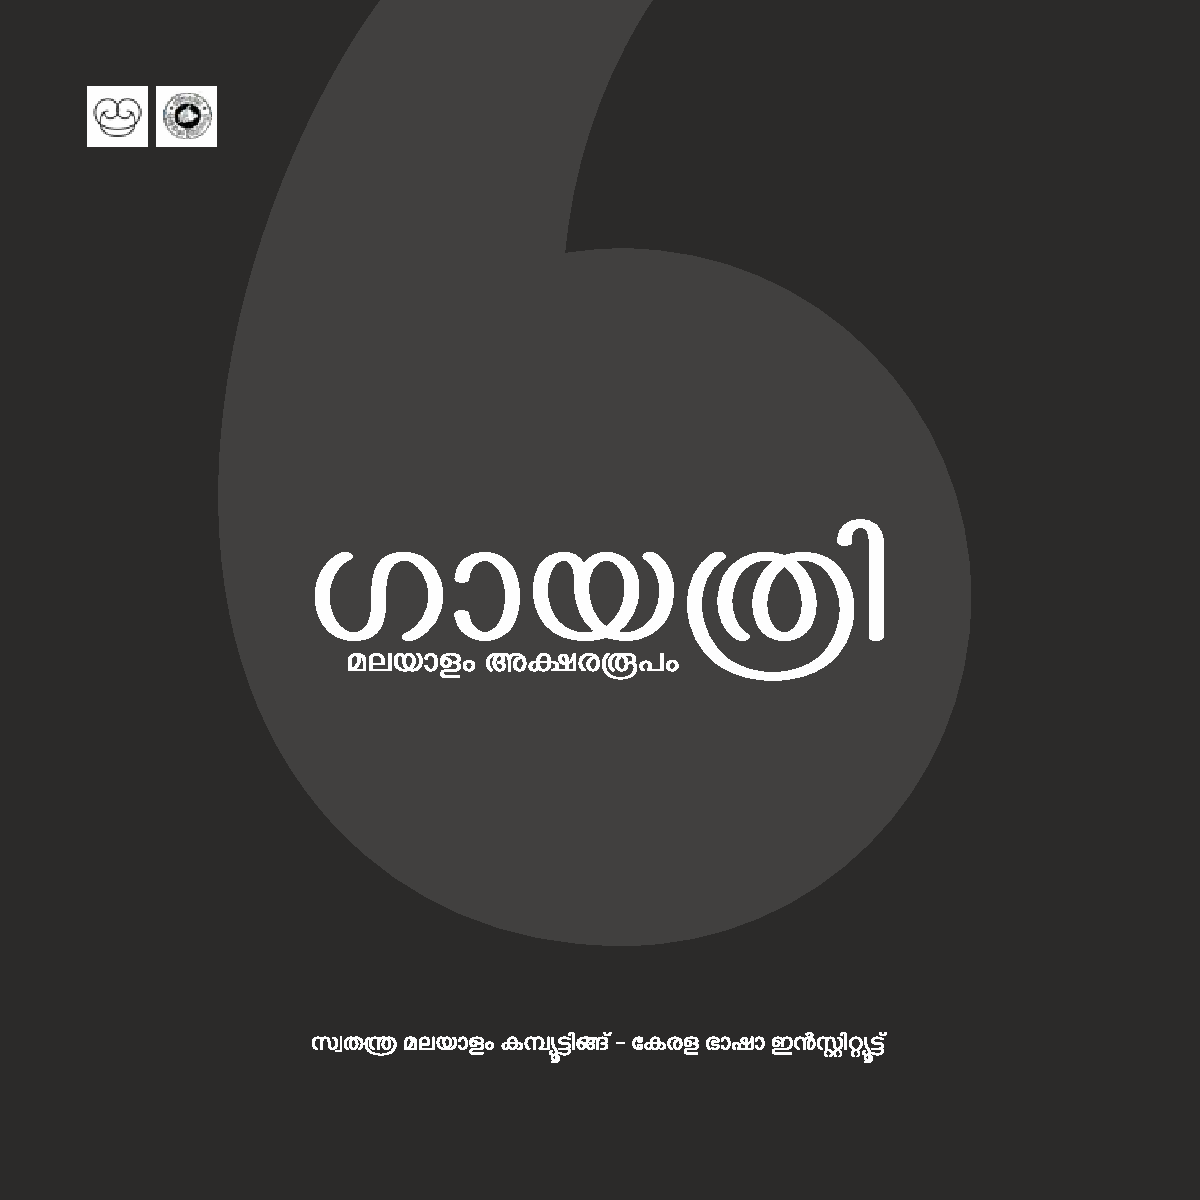
\includepdf[pages=-]{usecase.pdf}
	
	
	\chapter*{സാങ്കേതിക വിശദാംശങ്ങള്‍}
	
	ഗായത്രി ഫോണ്ടില്‍ ഉള്‍ക്കൊള്ളിച്ചിട്ടുള്ള മുഴുവന്‍ അക്ഷരങ്ങളേയും കുറിച്ചുള്ള വിശദാംശങ്ങൾ 
	
		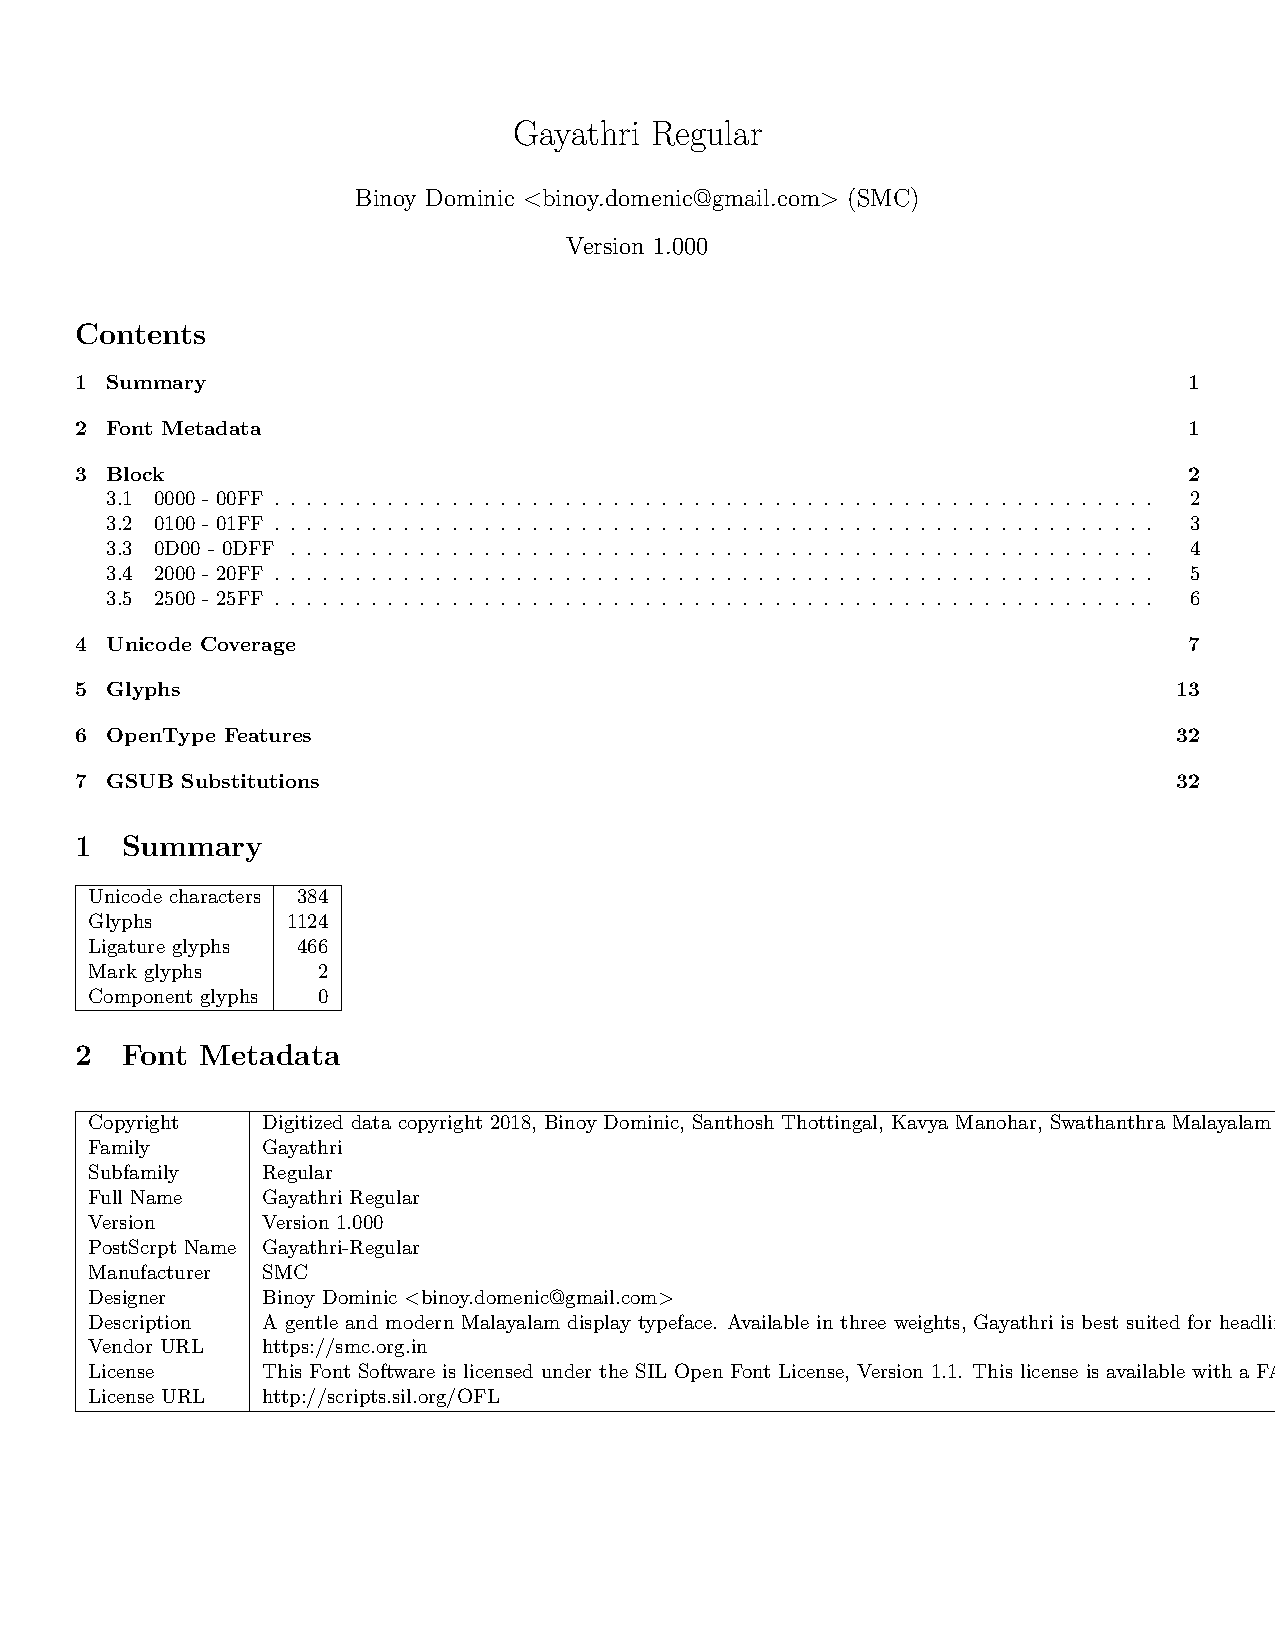
\includepdf[pages=-]{Gayathri.pdf}
	
	

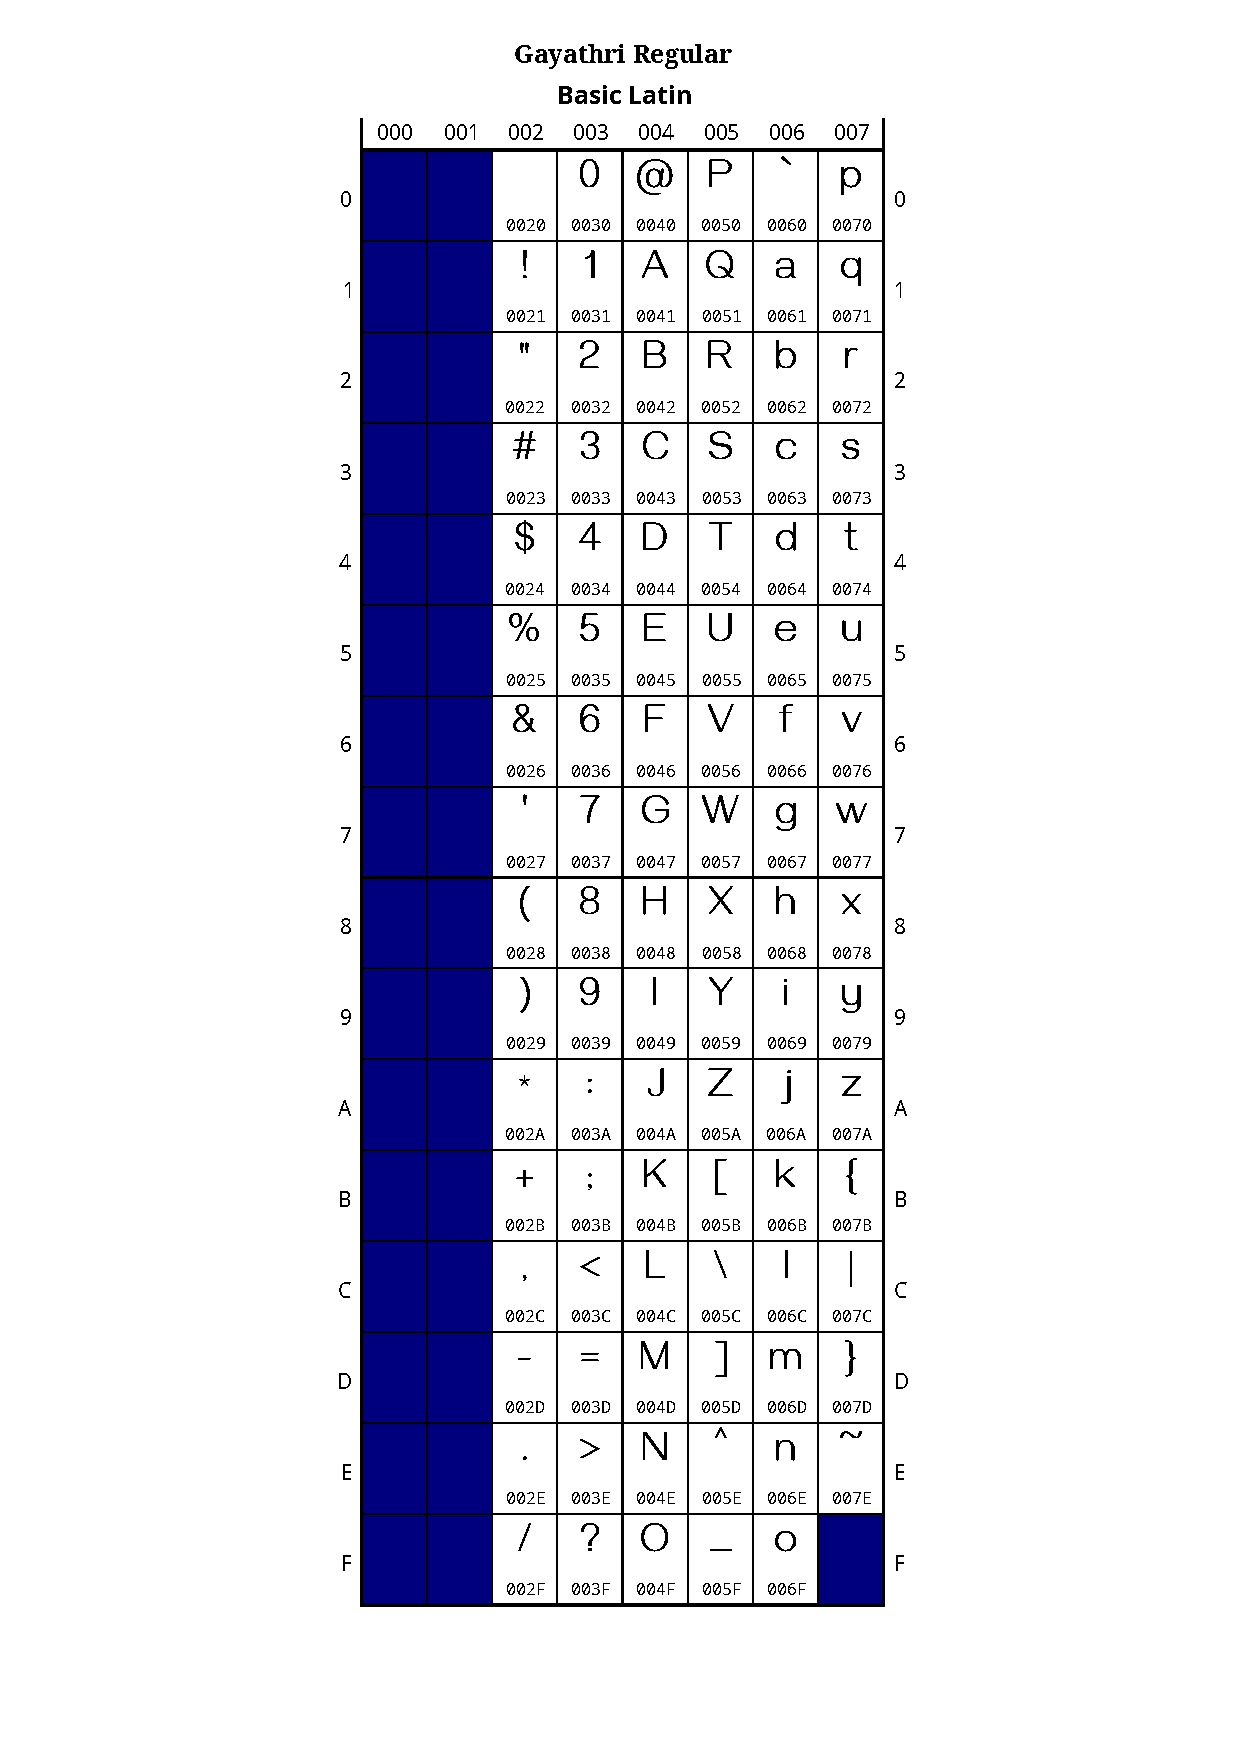
\includepdf[pages=-]{Gayathri-Regular-table.pdf}

	

	
\end{document}


 
